\section {Wstęp}
\subsection {Czym jest LIDAR ?}

Za wikipedią:
Lidar (od angielskiego akronimu LIDAR, utworzonego od wyrażenia: Light Detection and Ranging)
– urządzenie działające na podobnej zasadzie jak radar (Radio Detection and Ranging), ale
wykorzystujące światło lasera zamiast mikrofal. Urządzenie charakteryzuje się wysoką
rozdzielczością \cite{lidar_pl}.\\

Pierwsze użycie lasera do pomiaru odległości miało miejsce na potrzeby amerykańskiego 
wojska na początku lat 60, zaraz po wynalezieniu lasera. Było to użycie laserowego dalmierza 
model Colidar Mark II - obiekt, ze względu na swoje rozmiary, przypominał strzelbę \cite{lidar_en}.\\

Pierwsze zastosowanie urządzeń przypominających obecne Lidary to rok 1971 i działalność
Amerykańskiego Centrum Badań Fizyki Atmosfery w Boulder w Kolorado (National Center for
Atmospheric Research). Urządzenie dokonywało pomiaru wysokości chmur i zanieczyszczenia
atmosferycznego. Kolejne zastosowanie tego samego roku miało miejsce w czasie misji
Apollo 15 gdzie za pomocą sonaru laserowego (tak technologia ta była wówczas nazywana)
skanowano powierzchnię księżyca \cite{lidar_en}.\\

Ogólna zasada działania polega na połączeniu lasera z teleskopem. Laser wysyła, poprzez układ optyczny, bardzo krótkie i dokładnie wymierzone, ale silne impulsy elektromagnetyczne w widmie światła widzialnego lub podczerwonego. Na przebytym dystansie światło to ulega rozproszeniu, które jest obserwowane za pomacą teleskopu, fotodiody, fotopowielacza albo kamer CCD lub CMOS. \\

Zasadę te doskonale ilustruje rysunek z książki Paula McManamoma:
Figure 1.2 LiDAR Conceptual diagram (adapted from Ref. 3) \cite{mcmanamom}.\\
\begin{figure}[h]
    \centering
    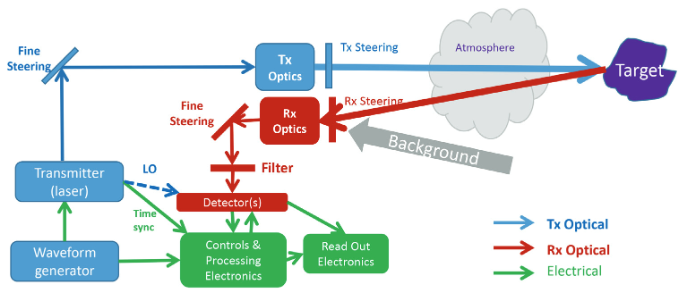
\includegraphics[scale=0.5]{lidar_concept}
    \caption{Rysunek z książki Paula McManamoma - LiDAR Conceptual diagram}
    \label{fig:lidar_concept}
\end{figure}

Dr. Pinliang Dong w swojej książce "LiDAR Remote Sensing and Applications" prezentuje wpływ zjawisk atmosferycznych na pomiary Lidaru \cite{dong}, jednak w mojej pracy pomiarów dokonywałem jedynie w pomieszczeniach zamkniętych (co z resztą sugerowała specyfikacja dalmierza TFmini Plus gdzie deklarowana przez producenta dokładność podana była dla pomieszczeń zamkniętych).\\

\subsection {Cel pracy}
Celem pracy jest zbudowanie działającej implementacji (zarówno sprzętowej jak i programowej) lidaru dwuwymiarowego za pomocą dalmierza laserowego oraz silnika krokowego. Te dwa urządzenia będą rdzeniem implementacji która za pośrednictwem mikrokontrolera będzie w stanie przekazać do komputera dane z których napisany przez nas program wygeneruje dwuwymiarowy obraz pomieszczenia.

\subsection {Współczesne zastosowanie lidarów}
Lidary mają dzisiaj szerokie zastosowanie: zarówno cywilne jak militarne. Technologia ta ma zastosowanie w architekturze, budownictwie, meteorologii, wywiadzie wojskowym i cywilnym, przemyśle produkcyjnym, na kolei czy w kartografii.\\

Pomimo że moja praca skupia się na podstawach działania i jest implementacją czysto amatorską, pragnąłbym przybliżyć nieco lepiej współczesne zastosowanie zaawansowanych technologicznie lidarów. Pozwoli to zrozumieć czemu technologia ta jest dziś tak ważna i dlaczego stanowi tak istotny element rozwoju wielu gałęzi gospodarki.\\

\subsubsection{Zastosowanie na kolei}
Ciekawym przypadkiem użycia lidarów jest zastosowanie przy inwentaryzacji i inspekcji torów kolejowym. Urządzenie skanujące umieszczone jest na frontowej części pociagu i dokonuje ciągłego skanowania zarówno torów, terenu jak i pozostałych elementów infrastruktury kolejowej (słupów, peronów, barierek a nawet całych stacji).\\

\begin{figure}[h]
    \centering
    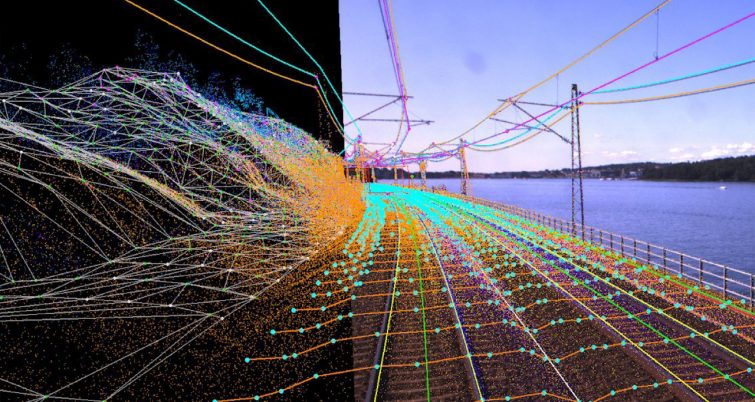
\includegraphics[scale=0.7]{LiDAR-AC-Image-1-755x402}
    \caption{Przykład skanu z artykułu: \cite{tory}}
    \label{fig:tory}
\end{figure}

Dzięki cyklicznym pomiarom i porównywaniu wyników system jest z stanie znaleźć nawet najdrobniejsze zmiany w terenie czy infrastrukturze. Pozwala to przewidzieć osiadanie terenu, odkształcenia torów czy uszkodzenia infrastruktury zanim jeszcze zmiany te okażą się krytyczne i staną się powodem usterek. Co więcej system jest w stanie przewidzieć np. optymalną prędkość (konfortową dla pasażerów) bądź uprzedać o istotnych niebezpiecznych zakrętach. System z powodzeniem stosowany w Wielkiej Brytanii, Francji czy Indiach.\\

Z laserowej inspekcji torów korzysta również nowojorskie metro.

\subsubsection{Zastosowanie budownictwie}
Zastosowanie w budownictwie jest bardzo szerokie natomiast kilka ciekawych rozwiązań posiada w swojej ofercie firma Leica. Serię BLK nazwałbym kamieniami milowymi współczesnego rozwoju technologii Lidar.\\

\textbf{BLK360}

\begin{figure}[h]
    \centering
    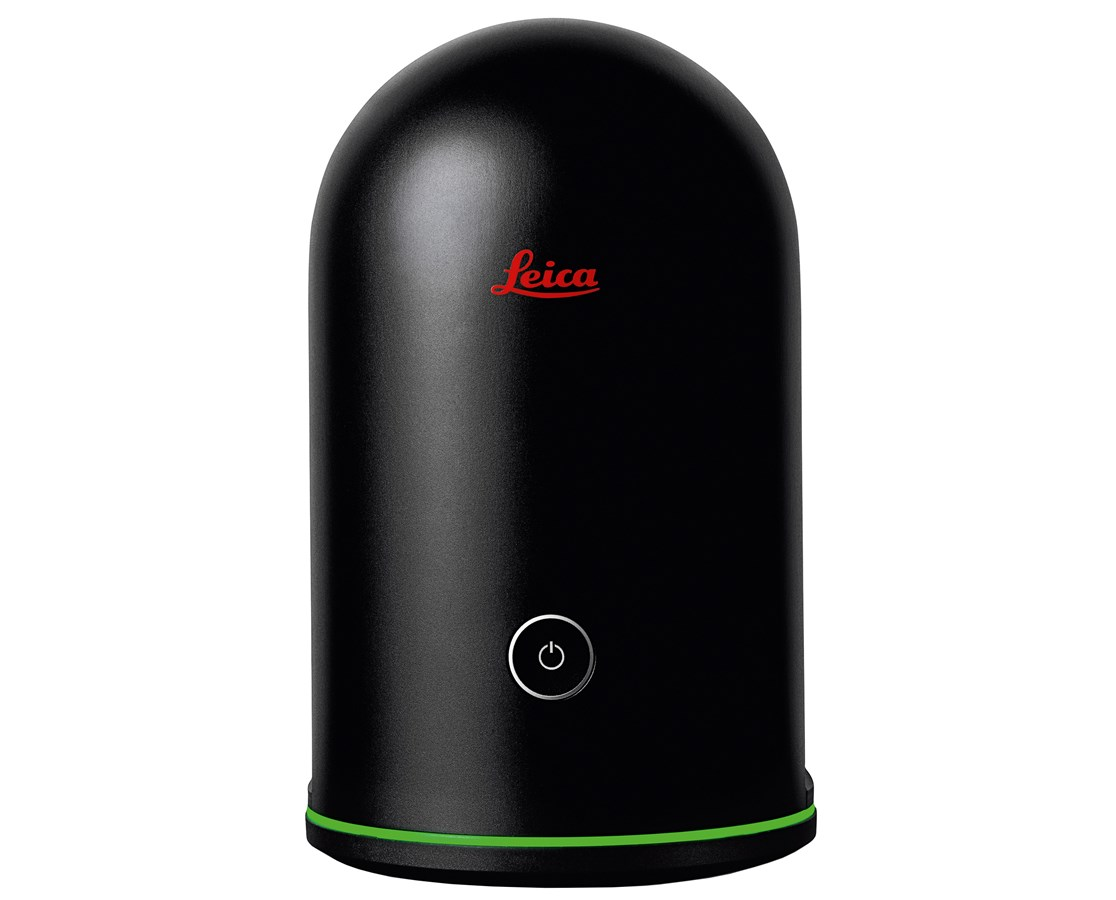
\includegraphics[scale=0.2]{Leica_BLK360_Front2}
    \caption{Frontowy panel urządzenia BLK360 \cite{blk360}}
    \label{fig:blk360}
\end{figure}

Urządzenie jest urządzniem statycznym. Zczytuje 360,000 punktów na sekundę z milimetrową dokładnością. Zasięg do 60 metrów. Dodatkowo rejestruje obraz z 3 kamer dzięki czemu możliwe jest również zastosowanie sztucznej inteligencji (głównie technologii \textbf{Uczenia Maszynowego}) do rozpoznawania obiektów w budynku (okna, drzwi, instalacje) i tworzenia interaktywnego modelu \textbf{BIM (Building Information Modeling)}.\\

\textbf{BLK2GO}

Mobilna i ulepszona wersja BLK360. Pozwala tworzyć modele całych budynków w czasie rzeczywistym. Dodatkowo również obsługuje rozpoznawanie elementów budynku i tworzy model BIM.\\
\begin{figure}[h]
    \centering
    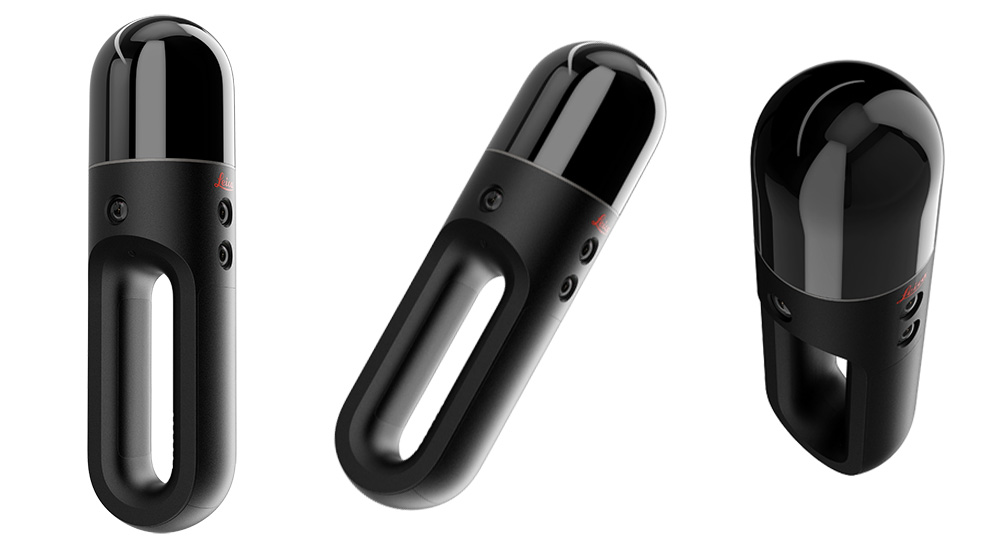
\includegraphics[scale=0.4]{blk2go}
    \caption{Frontowy panel urządzenia BLK2GO \cite{blk2go}}
    \label{fig:blk2go}
\end{figure}

\textbf{BLK2FLY}

\begin{figure}[h]
    \centering
    \includegraphics[scale=0.4]{blk2fly}
    \caption{Render planowanego wyglądu urządzenia \cite{blk2fly}}
    \label{fig:blk2fly}
\end{figure}

We wrześniu 2021 roku pojawił się oficjalny komunikat firmy Leica dotyczący kolejnego projektu - \textbf{BLK2FLY}. Urządzenie wykorzystuje drona i jest w pełni autonomiczne. Użytkownik, na urządzeniu mobilnym, wybiera jedynie porządany obiekt (np. cały budynek) a automatycznie sterowany drone samodzielnie dokonuje wszyskich zadanych pomiarów. Ogromna mobilność drona pozwala na pomiar trudno dostępnych dla człowieka miejsc.\\

\textbf{BLK247}\\
System monitoringu przemysłowego który prócz technologii Lidar wykorzystuje jeszcze obraz wideo i pomiar temperatury powierzchni.\\
\begin{figure}[h]
    \centering
    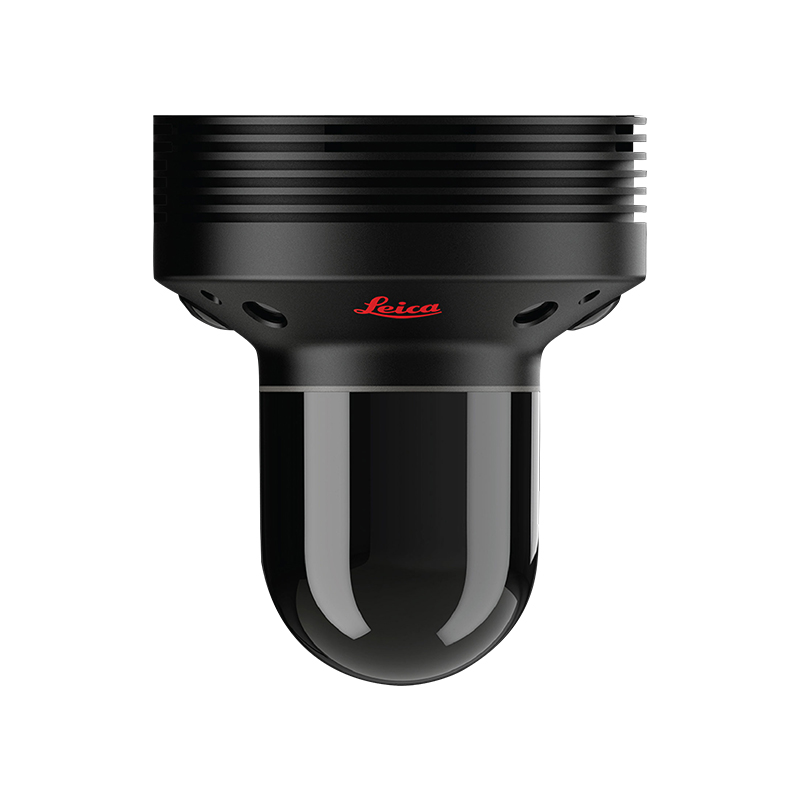
\includegraphics[scale=0.3]{BLK247}
    \caption{Pojedyncza kamera systemu BLK247 \cite{blk247}}
    \label{fig:blk247}
\end{figure}
Przewagę nad systemami monitoringu wykorzystującymi jedynie kamery jest taka że system jest w stanie tworzyć obraz i wykrywać ruch nawet przy całkowitej ciemności. Dodatkowo system termowizyjny wykrywa ludzi i zwierzęta a technologie AI pozwalają klasyfikować wykrywane obiekty.

\begin{figure}[h]
    \centering
    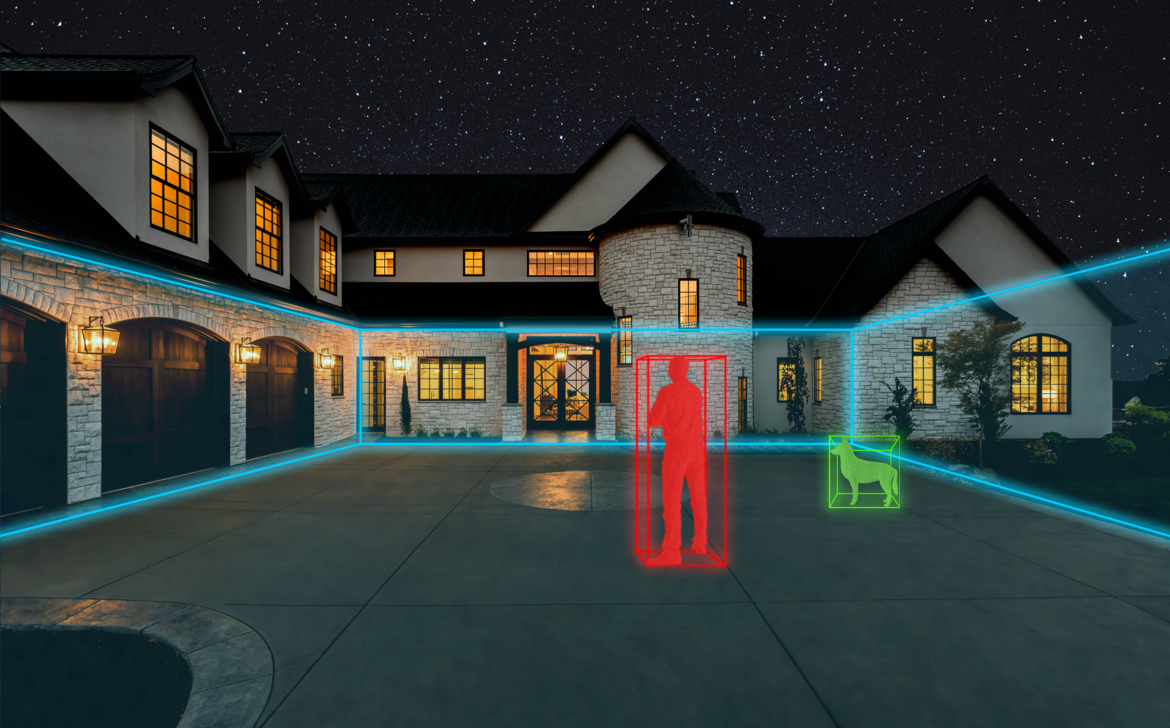
\includegraphics[scale=0.3]{BLK247-house-night_0}
    \caption{Poglądowy schemat działania ze strony internetowej producenta \cite{blk247}}
    \label{fig:house-night}
\end{figure}


